% !TEX TS-program = XeLaTeX
% use the following command:
% all document files must be coded in UTF-8
\documentclass[spanish]{textolivre}
% build HTML with: make4ht -e build.lua -c textolivre.cfg -x -u article "fn-in,svg,pic-align"
%\usepackage{longtable}
\usepackage{graphicx}
\usepackage{array}
\usepackage{caption}   % Para legendas
\usepackage{float}

\journalname{Texto Livre}
\thevolume{18}
%\thenumber{1} % old template
\theyear{2025}
\receiveddate{\DTMdisplaydate{2025}{1}{9}{-1}} % YYYY MM DD
\accepteddate{\DTMdisplaydate{2025}{2}{6}{-1}}
\publisheddate{\DTMdisplaydate{2025}{6}{1}{-1}}
\corrauthor{Antonio León Garrido}
\articledoi{10.1590/1983-3652.2025.56904}
%\articleid{NNNN} % if the article ID is not the last 5 numbers of its DOI, provide it using \articleid{} commmand 
% list of available sesscions in the journal: articles, dossier, reports, essays, reviews, interviews, editorial
\articlesessionname{articles}
\runningauthor{León Garrido y Barroso-Osuna} 
%\editorname{Leonardo Araújo} % old template
\sectioneditorname{Hugo Heredia Ponce}
\layouteditorname{Saula Cecília}

\title{Evaluación de apps y diseño de un recurso tecnológico para el aprendizaje de la música}
\othertitle{Avaliação de aplicações e concepção de um recurso tecnológico para a aprendizagem de música}
% if there is a third language title, add here:
\othertitle{Evaluation of apps and design of a technological resource for learning music}

\author[1]{Antonio León-Garrido~\orcid{0000-0002-4850-596X}\thanks{Email: \href{mailto:aleon@us.es}{aleon@us.es}}}
\author[1]{Julio Manuel Barroso-Osuna~\orcid{0000-0002-4850-596X}\thanks{Email: \href{mailto:jbarroso@us.es}{jbarroso@us.es}}}
\affil[1]{Universidad de Sevilla, Facultad de Ciencias de la Educación, Departamento de Didáctica y Organización Educativa, Sevilla, Andalucía, España.}

\addbibresource{article.bib}
% use biber instead of bibtex
% $ biber article

% used to create dummy text for the template file
%\definecolor{dark-gray}{gray}{0.35} % color used to display dummy texts
%\usepackage{lipsum}
%\SetLipsumParListSurrounders{\colorlet{oldcolor}{.}\color{dark-gray}}{\color{oldcolor}}

% used here only to provide the XeLaTeX and BibTeX logos
%\usepackage{hologo}

% if you use multirows in a table, include the multirow package
%\usepackage{multirow}

% provides sidewaysfigure environment
%\usepackage{rotating}

% CUSTOM EPIGRAPH - BEGIN 
%%% https://tex.stackexchange.com/questions/193178/specific-epigraph-style
%\usepackage{epigraph}
%\renewcommand\textflush{flushright}
%\makeatletter
%\newlength\epitextskip
%\pretocmd{\@epitext}{\em}{}{}
%\apptocmd{\@epitext}{\em}{}{}
%\patchcmd{\epigraph}{\@epitext{#1}\\}{\@epitext{#1}\\[\epitextskip]}{}{}
%\makeatother
%\setlength\epigraphrule{0pt}
%\setlength\epitextskip{0.5ex}
%\setlength\epigraphwidth{.7\textwidth}
%% CUSTOM EPIGRAPH - END

% to use IPA symbols in unicode add
%\usepackage{fontspec}
%\newfontfamily\ipafont{CMU Serif}
%\newcommand{\ipa}[1]{{\ipafont #1}}
% and in the text you may use the \ipa{...} command passing the symbols in unicode

% LANGUAGE - BEGIN
% ARABIC
% for languages that use special fonts, you must provide the typeface that will be used
% \setotherlanguage{arabic}
% \newfontfamily\arabicfont[Script=Arabic]{Amiri}
% \newfontfamily\arabicfontsf[Script=Arabic]{Amiri}
% \newfontfamily\arabicfonttt[Script=Arabic]{Amiri}
%
% in the article, to add arabic text use: \textlang{arabic}{ ... }
%
% RUSSIAN
% for russian text we also need to define fonts with support for Cyrillic script
% \usepackage{fontspec}
% \setotherlanguage{russian}
% \newfontfamily\cyrillicfont{Times New Roman}
% \newfontfamily\cyrillicfontsf{Times New Roman}[Script=Cyrillic]
% \newfontfamily\cyrillicfonttt{Times New Roman}[Script=Cyrillic]
%
% in the text use \begin{russian} ... \end{russian}
% LANGUAGE - END

% EMOJIS - BEGIN
% to use emoticons in your manuscript
% https://stackoverflow.com/questions/190145/how-to-insert-emoticons-in-latex/57076064
% using font Symbola, which has full support
% the font may be downloaded at:
% https://dn-works.com/ufas/
% add to preamble:
% \newfontfamily\Symbola{Symbola}
% in the text use:
% {\Symbola }
% EMOJIS - END

% LABEL REFERENCE TO DESCRIPTIVE LIST - BEGIN
% reference itens in a descriptive list using their labels instead of numbers
% insert the code below in the preambule:
%\makeatletter
%\let\orgdescriptionlabel\descriptionlabel
%\renewcommand*{\descriptionlabel}[1]{%
%  \let\orglabel\label
%  \let\label\@gobble
%  \phantomsection
%  \edef\@currentlabel{#1\unskip}%
%  \let\label\orglabel
%  \orgdescriptionlabel{#1}%
%}
%\makeatother
%
% in your document, use as illustraded here:
%\begin{description}
%  \item[first\label{itm1}] this is only an example;
%  % ...  add more items
%\end{description}
% LABEL REFERENCE TO DESCRIPTIVE LIST - END


% add line numbers for submission
%\usepackage{lineno}
%\linenumbers

\begin{document}
\maketitle

\begin{polyabstract}
\begin{abstract}
El crecimiento constante de las apps móviles y su integración en la educación han generado interrogantes sobre la calidad y la adecuación a los contextos educativos. En este estudio, se evaluaron apps móviles destinadas al aprendizaje de la Educación Musical mediante un instrumento de evaluación específico. Además, se analizaron las posibles diferencias entre los expertos en tecnología educativa y música, frente a aquellos especializados únicamente en música. Participaron 60 docentes especialistas en Educación Musical, de los cuales 28 pertenecían a instituciones universitarias y 32 a centros educativos de Educación Primaria. Los resultados mostraron un alto índice de concordancia en las evaluaciones (CCI = 0.957) y una media ponderada de 3.5 sobre 5 puntos para las apps analizadas. Además, no se encontraron diferencias estadísticamente significativas entre los grupos evaluadores, lo que sugiere una consistencia en los criterios de valoración. Estos hallazgos resaltan la importancia de evaluar y desarrollar apps móviles educativas con base en criterios de calidad definidos y orientados a la educación. Por estos motivos, se concluye proponiendo una nueva app móvil que integra características de calidad identificadas en el análisis. Esta nueva app representa un aporte significativo para la enseñanza de la música, contribuyendo a mejorar los resultados educativos mediante el uso de la tecnología y fomentar el aprendizaje de forma significativa. 

\keywords{Apps móviles\sep Evaluación \sep TIC\sep Educación Musical\sep Propuesta diseño}
\end{abstract}

\begin{portuguese}
\begin{abstract}
O crescimento constante das aplicações móveis e a sua integração na educação têm levantado questões sobre a qualidade e adequação aos contextos educativos. Neste estudo, aplicativos móveis voltados para a aprendizagem da Educação Musical foram avaliados por meio de um instrumento de avaliação específico. Além disso, foram analisadas as possíveis diferenças entre especialistas em tecnologia educacional e música, em comparação com aqueles especializados apenas em música. Participaram 60 professores especializados em Educação Musical, dos quais 28 pertenciam a instituições universitárias e 32 a centros educativos do Ensino Básico. Os resultados mostraram uma alta taxa de concordância nas avaliações (CCI = 0,957) e uma média ponderada de 3,5 de 5 pontos para os aplicativos analisados. Além disso, não foram encontradas diferenças estatisticamente significativas entre os grupos de avaliação, sugerindo uma consistência nos \textit{endpoints}. Esses resultados destacam a importância de avaliar e desenvolver aplicações móveis educativas com base em critérios de qualidade definidos e orientados para a educação. Por essas razões, concluímos propondo uma nova aplicação móvel que integra características de qualidade identificadas na análise. Essa nova aplicação representa um aporte significativo para o ensino da música, contribuindo para melhorar os resultados educativos através da utilização da tecnologia e promovendo a aprendizagem de uma forma significativa. 

\keywords{Aplicações móveis\sep Avaliação\sep TIC\sep Educação musical\sep Proposta de design}
\end{abstract}
\end{portuguese}

\begin{english}
\begin{abstract}
The constant growth of mobile apps and their integration into education have raised questions about quality and suitability for educational contexts. In this study, mobile apps aimed at learning music education were evaluated using a specific evaluation instrument. Additionally, possible differences between experts in educational technology and music, compared to those specialised only in music, were analysed. Sixty teachers specialising in music education participated, of whom 28 belonged to university institutions and 32 to primary education centres. The results showed a high rate of agreement in the evaluations (CCI = 0.957) and a weighted average of 3.5 out of 5 points for the apps analysed. Furthermore, no statistically significant differences were found between the evaluation groups, suggesting consistency in the endpoints. These findings highlight the importance of evaluating and developing educational mobile apps based on defined and education-orientated quality criteria. For these reasons, we conclude by proposing a new mobile app that integrates the quality characteristics identified in the analysis. This new app represents a significant contribution to the teaching of music, contributing to improving educational results through the use of technology, and promoting learning in a significant way.

\keywords{Mobile apps\sep Evaluation\sep ICT\sep Music education\sep Design proposal}
\end{abstract}
\end{english}
% if there is another abstract, insert it here using the same scheme
\end{polyabstract}

\section{Introducción}\label{sec-intro}
El \textit{mobile learning}, entendido como el aprendizaje a través de los dispositivos móviles, ha experimentado un crecimiento exponencial en los últimos años, convirtiéndose en una de las principales tendencias en los contextos educativos para facilitar los procesos de enseñanza-aprendizaje \cite{cuevas-montero2024}. Esta expansión ha impulsado el desarrollo de apps móviles educativas dirigidas a diferentes disciplinas, incluyendo la Educación Musical. Sin embargo, la gran cantidad de apps disponibles no garantiza su calidad ni su adecuación pedagógica, lo que plantea la necesidad de contar con ciertos mecanismos de evaluación de forma rigurosa, permitiendo analizar su impacto real en la enseñanza-aprendizaje. Y, a raíz de esta integración, han surgido diversas investigaciones sobre el uso de los smartphones en la educación \cite{romero-rodriguez2023, lerma-noriega2023}. Sin embargo, la mayoría de estos estudios se han centrado en analizar la eficacia y la seguridad de estas herramientas, dejando en un segundo plano el análisis de su calidad.

El uso de las apps en la enseñanza de la música ha demostrado múltiples beneficios, como el desarrollo de la creatividad, la mejora y el desarrollo de la memoria auditiva y el fortalecimiento de las habilidades prácticas en la música  \cite{akombo2019, cheng2023, han2023, barroso-osuna2024}. No obstante, muchos de los recursos tecnológicos digitales han sido diseñados sin la validación pedagógica, en la que se prioriza aspectos técnicos o simplemente comerciales sin tener en cuenta los criterios didácticos esenciales \cite{hirsh-pasek2015, merchant2020}. 

En el caso de la Educación Musical, la evaluación de las apps debe ser más crucial, ya que las apps móviles diseñadas para este campo no solo proporcionan un contenido teórico-práctico, sino que también facilitan el desarrollo de habilidades musicales esenciales para el aprendizaje y el desarrollo cognitivo \cite{dominguez-lloria2023, meneses-rodriguez2024}. Estos aspectos parten de diversos estudios que han demostrado que la tecnología implementada de forma correcta en la enseñanza de la música ayuda a mejorar el rendimiento académico y la motivación de los estudiantes \cite{vela-gonzalez2020, riano2022}, siempre y cuando se utilice de manera adecuada, contribuirá a mejorar el aprendizaje de la música de forma significativa \cite{aufegger2020, joseph2023}. No obstante, existen la falta de criterios homogeneizados para evaluar la calidad de las apps móviles que contribuyen al aprendizaje de cualquier materia \cite{delgado-morales2023, quezada-bolanos2023}.

Por otro lado, la percepción de la calidad de las apps puede presentar variaciones en función del evaluador. De hecho, mientras que los especialistas en TIC pueden centrarse en aspectos más técnicos y centrados en el diseño de las apps, los docentes de música pueden priorizar la precisión y relevancia de los contenidos didácticos que se han integrado. Es por ello que conocer las posibles diferencias significativas entre los dos perfiles resulta interesante para comprender cómo distintos enfoques pueden influir en la evaluación de los recursos tecnológicos, así como la integración fructífera en el aula. Por tanto, se podría decir que la evaluación de la tecnología contribuirá una mayor seguridad en la educación, flexibilidad del contenido y dinamización del aprendizaje \cite{uribe-guerrero2023}. No obstante, aunque el uso de las apps contribuye a mejorar la educación, también puede implicar una serie de riesgos como la dependencia excesiva o la falta de contenido pedagógicos por no cumplir con los estándares de privacidad o accesibilidad, afectando negativamente al aprendizaje \cite{joseph2023}. 

Por ende, la presente investigación se justifica por la necesidad de contar con un análisis riguroso de las apps móviles destinadas al aprendizaje de la Educación Musical, con el propósito de asegurar que estas herramientas ayudan a favorecer el aprendizaje, cumpliendo con estándares de calidad adecuados. La evaluación de estos recursos permitirá contribuir al diseño y desarrollo de nuevas apps, garantizando que responde a las necesidades de los contextos educativos actuales \cite{quezada-bolanos2023}.

A partir de las aportaciones realizadas, se plantearon los siguientes objetivos de investigación: 

\begin{itemize}
  \item Evaluar apps móviles diseñadas al aprendizaje de la Educación Musical básica mediante un instrumento de evaluación específico que permita medir su calidad.
  \item Analizar si existen diferencias significativas entre los dos grupos de docentes evaluadores: especialistas en TIC y Educación Musical versus especialistas solo en música. Para ello, se establecieron las siguientes hipótesis para contrastarlas:
  \begin{itemize}
    \item H0 (hipótesis nula): no existen diferencias significativas entre los grupos evaluadores;
    \item H1 (hipótesis alternativa): existen diferencias significativas entre los grupos evaluadores;
  \end{itemize}
  \item Proponer una nueva app para el aprendizaje de Educación Musical básica para las primeras etapas educativas de iniciación, basada en los datos obtenidos, con el fin de contribuir al desarrollo de nuevas herramientas tecnológicas en la educación musical para optimizar la enseñanza.
\end{itemize}

\subsection{Evaluación de las apps móviles en la educación}\label{sec-normas}
El \textit{mobile learning} ha impulsado diversas investigaciones sobre el uso de los smartphones en la educación \cite{romero-rodriguez2023, lerma-noriega2023}. Sin embargo, la mayoría de los estudios se ha centrado en analizar la eficacia y la seguridad de las mismas sin analizar el punto más importante para la educación, la calidad. 

Según \textcite{gomez2020}, los desarrolladores de apps móviles consideran ciertas variables educativas para garantizar una tecnología de calidad, prestando especial atención a aspectos como el contenido, la estética y la usabilidad técnica. Estos factores pueden influir en la percepción de los usuarios en tan solo 50 milisegundos \cite{joachims2017}. En estas líneas, se debe tener presente los estudios recientes que han enfatizado la importancia de establecer criterios de evaluación rigurosos para analizar la calidad de las apps educativas como los de \textcite{hirsh-pasek2015, merchant2020}. No obstante, existen la falta de criterios homogeneizados para evaluar la calidad de las apps móviles que contribuyen al aprendizaje de cualquier materia \cite{delgado-morales2023, quezada-bolanos2023}.

Por otro lado, mientras que los especialistas en tecnología educativa priorizan mejorar los aspectos técnicos y el diseño de los recursos tecnológicos, los docentes de música se centran en la precisión y aplicación de la didáctica de la música para que los alumnos desarrollen las habilidades y destrezas musicales. En este sentido, conocer los diversos enfoques pueden influir en la evaluación de las apps y resulta en un aspecto importante para mejorar la integración de las apps en los contextos educativos \cite{eusterbrock2023, quezada-bolanos2023}.

\section{Método}\label{sec-2}
El presente estudio se enmarca en un enfoque cuantitativo y correlacional. La población estuvo compuesta por docentes especialistas en música de ámbitos universitarios y de centros de estudios de Educación Primaria en activo, con más de dos años de experiencia docente. La selección de la muestra se realizó mediante un muestreo intencionado, no probabilístico y por conveniencia, obteniendo un total de $N$ = 60 participantes. 

De estos, 28 docentes (46,7\%) son especialistas en universidad, formando a los futuros docentes de magisterio, de los cuales 8 (28,58\%) eran hombres y 20 (71,42\%) mujeres. Por otro lado, 32 docentes (53,3\%) eran maestros de centros de Educación Primaria, con 20 (62,5\%) hombres y 12 (37,5\%) mujeres. En términos generales, la muestra estuvo conformada por 28 hombres (46,7\%) y 32 mujeres (53,3\%). La edad media de la población oscilaba entre 27 a 47 años, con una media de 38,27 años, con una desviación estándar (DT) de 6,393 y error de media de 0,825.

Además, del cómputo total de docentes, 27 (45\%) eran especialistas en el campo de las TIC aplicadas a la Educación Musical, mientras que 33 (55\%) no son especialistas en las TIC, sino solo en música. Para determinar el nivel de experticia en ambos campos, se utilizó el Cálculo del Coeficiente de Competencia Experta, siguiendo la metodología recomendada por \textcite{cabero-almenara2020, herrera2023}. Fueron considerados expertos aquellos docentes que obtuvieron un valor igual o superior al 0.8, mientras que los no expertos en TIC se situaron en un rango entre 0.55 y 0.75, lo que indica un cierto conocimiento en TIC aplicadas a la música, pero insuficiente para considerarlos expertos en ambos campos.  

Los especialistas en TIC y Educación Musical estuvieron compuestos por 17 docentes universitarios (60.7\%) y 10 docentes de Educación Primaria (31,25\%). Mientras que los 11 docentes universitarios (39.3\%) y 22 docentes de Educación Primaria (68,75\%) eran especialistas exclusivamente en música.

Para la selección de muestra de apps, se establecieron los siguientes criterios: sistema operativo Android; integración de contenidos relacionados con la lectoescritura musical, la formación rítmica o la formación auditiva, para el aprendizaje musical básico; acceso gratuito o en la modalidad de prueba; valoración mínima de 3.5 estrellas en Google Play, o, en su defecto, ausencia de valoraciones si la app fue lanzada en 2024; preferencia de apps en español, y seguida de otros idiomas. Con base en estos criterios, se identificaron 107 apps de las cuales se seleccionaron aleatoriamente 60 para su evaluación.

A continuación, en la Tabla \ref{tab-1} se muestra la relación de apps seleccionadas junto con sus versiones correspondientes. 

\begin{longtable}{p{7cm} p{4cm} p{2cm}}
\caption{Relación de apps seleccionadas para la investigación.}\label{tab-1} \\
\toprule
Muestra de apps & Versión & Valoración \\
\midrule
\endhead

Aprendo música & 0.51 & 4.6 \\
Asistente teoría musical & V5.1.4 & 3.9 \\
Caja de ritmos -- Groovepad, Beat & 1.4.1 & 4 \\
ChordIQ & 3.2.612 & 4.4 \\
Complete Ear Trainer & 2.6.1-169 & 4.8 \\
Complete Music Reading Trainer & 1.6.2-104 & 4.7 \\
Complete Rhythm Trainer & 1.6.2-109 & 4.7 \\
Coryvo -- Entrenador de ritmo & 4.2.7 & x \\
Curso para leer música & 1.0.53 & 4.5 \\
DoReMi Music Academy & 1.4.03 & 4.4 \\
DoReMiNotas & 1.09 & 4.4 \\
DoReMiNotas Plus Leer Música & x & x \\
Drum Pad Machine & 2.25.0 & 4.4 \\
Ear master -- lectura de notas & 7.5.68 & 4.5 \\
Ear Trainer -- Perfect ear & 3.9.74 & 4.7 \\
Ear Training -- Prueba de Ritmo & 1.0.13 & x \\
Ear training Rhythm & 1.0.15 & x \\
EarForge: Learn Ear Training & 5.5.0 & x \\
Rhythm Trainer & 0.2302051943 & 4.8 \\
Entrenamiento Auditivo & 1.0.69 & 4.1 \\
Entrenamiento auditivo básico & 1.0.39 & x \\
Entrenamiento Auditivo- Rítmico & 1.0.15 & x \\
Entrenar oído musical & 4.3 & 3.8 \\
Escala acordes y progresiones & P-Rate-US\_fix & 4.9 \\
Funcional Ear trainer & 3.12.6 & 4.8 \\
Groovepad -- creador de música & 1.22.0 & 4.7 \\
Groovy Loops & 1.21.1 & 3.9 \\
Intervalos: test oído musical & 1.3 & x \\
Kids Music Lite & 1.2.4 & x \\
La Abeja Maya: Música & 0.32 & 3.9 \\
Learn Music Notes Sight Read & 1.4.1 & 4.2 \\
Leer música & 1.0.105 & 4.0 \\
Leer notas musicales & 7.05 & 4.3 \\
Leitura de partitura -- Jogo & 1.3 & x \\
Magic Tiles 3 & 11.022.107 & 3.8 \\
Meludia Melody & 1.15.14 & 3.7 \\
Music Interval Ear Training & 1.4.1 & x \\
Music Note Reading & 7.0.2 & x \\
Music Reading Trainer & 1.04 & 4.5 \\
Music Theory Learn Notes Chord & 1.0.56 & 4 \\
Music tutor (sight Reading) & 2.28 & 4.2 \\
Musical Ear Training -- Theory & 19 & 5 \\
MyEarTraining -- Ear Training & 3.8.2.0 & 4.8 \\
MyMusic Theory & 2.4.6 & 4.7 \\
Note Rote: Music reading tutor & x & x \\
Noten Lernen & 1.8.1 & x \\
Notes de musique & 8.4 & 4.6 \\
NoteTeacher & 1.5.3 & 4.3 \\
Oído musical: Tono absoluto. & 1.2 & 3.9 \\
Piano Sight Reading Trainer & 4.3.0 & 4.0 \\
Polyrhythm -- Rhythm Trainer & 1.2.3 & 4.9 \\
Rhythmic Village & 2.19.28 & 4.7 \\
Ritmo a Puntas & 2.4.1 & 3.6 \\
Saber leer notas musicales & 1.0.82 & 4.3 \\
Solfaread & 1.2 & 4.5 \\
Solfeador & 3.0.1 & 4.5 \\
Solfeo & 1.09 & 4.3 \\
The Ear Gym & 4.2.1 & 4.8 \\
Treine Partitura e Ouvido & 1.1 & 3.8 \\
Vivo -- aprender notas musicales & 1.3.9 & x \\
\bottomrule
\source{Elaboración propia.}
\end{longtable}


\subsection{Instrumento de recogida de datos}\label{sec-2_1}
Para la evaluación de las apps móviles, se utilizó el instrumento de recogida de datos desarrollado por \textcite{leon-garrido2024} diseñado específicamente para valorar apps móviles destinadas al aprendizaje de la Educación Musical. Esta herramienta fue desarrollada tomando como referencia estudios previos sobre la evaluación de la tecnología educativa y modelos específicos para la valoración de apps en el ámbito educativo. El instrumento consta de un total de 70 ítems organizado en dos partes:

\begin{itemize}
    \item Primera parte: Elementos de identificación (39 ítems), que permite conocer las características básicas de la app evaluada.
    \item Segunda parte: Evaluación de la calidad: estructurada en tres dimensiones:
    \begin{itemize}
        \item Dimensión técnica-estética (10 ítems) enfocada en la calidad técnica visual de la app.
        \item Dimensión pedagógica-funcional (12 ítems) se centra en aspectos didácticos esenciales para facilitar el proceso de enseñanza-aprendizaje.
        \item Dimensión musical (9 ítems), analiza la calidad y cantidad de contenidos musicales incorporados en la app.
    \end{itemize}
\end{itemize}

Para garantizar la validez del contenido, se realizó un proceso de validación mediante juicio de expertos con la participación de especialistas en diferentes campos, especialmente en el campo de la tecnología educativa y la música, participando un total de 38 especialistas de diversas universidades del territorio español. Este instrumento obtuvo una valoración de 3.5 sobre 5 puntos.

\subsection{Procedimiento de recogida de datos}\label{sec-2_2}
Para el desarrollo de la investigación, se estableció contacto con docentes universitarios especializados en Educación Musical y con maestros de Educación Primaria con la mención en Educación Musical. Se llevó a cabo una sesión teórica sobre la aplicación de las apps móviles a la Educación Musical, seguida de una fase práctica donde los docentes exploraron las diversas apps seleccionadas para familiarizarse con sus funcionalidades.

Posteriormente, se presentó el instrumento de evaluación de apps móviles de \textcite{leon-garrido2024}, explicando cada ítem en detalle antes de proceder a la evaluación. Antes de iniciar la fase de evaluación, se calculó el Coeficiente de Competencia Experta para conocer el número de expertos en TIC y Música, a través de la fórmula \begin{math} K = \frac{1}{2}(Kc + Ka)\end{math}
donde $Kc$ es el coeficiente del conocimiento y $Ka$ el coeficiente de argumentación determinado por los rangos alto, medio y bajo \cite{cabero-almenara2020, herrera2023}. Datos que quedaron reflejados en la descripción de los participantes. 

Con el objetivo de evaluar la confiabilidad entre los docentes respecto a una misma aplicación móvil para el aprendizaje de la música, antes de evaluar las 60 apps móviles, se les proporcionó un recurso común para que interactuaran con la app y realizaran la evaluación de manera individual. Este estudio, recogido en \textcite{leon-garrido2025a}, analizó el nivel de acuerdo entre los evaluadores sobre una aplicación móvil diseñada para la enseñanza musical básica, distinta de las seleccionadas en la presente investigación. Para esta ocasión, se empleó la app Clefs. En dicha investigación, se utilizó el mismo instrumento de evaluación descrito previamente y se aplicaron el Coeficiente de Correlación Interclases (CCI), para medir la consistencia y fiabilidad de las evaluaciones, y la prueba ANOVA de Friedman, con el propósito de identificar diferencias significativas en las valoraciones. Los resultados indicaron un alfa de fiabilidad de 0.959, evidenciando una alta consistencia interna del instrumento. En cuanto al CCI, se obtuvieron valores elevados en las dimensiones técnica-estética (0.888), pedagógica-funcional (0.947) y musical (0.913), lo que sugiere un excelente nivel de acuerdo entre los evaluadores. Estos hallazgos respaldaron la fiabilidad del instrumento de evaluación y la consistencia en la calidad de la app, demostrando un alto nivel de concordancia entre los docentes en la valoración de un mismo recurso tecnológico.

Tras este estudio, cada docente descargó aleatoriamente una de las apps móviles seleccionadas para interactuar nuevamente con ella y proceder a su evaluación utilizando el instrumento previamente presentado. Se decidió que cada docente evaluara una única aplicación, dado el alto nivel de acuerdo observado en estudios previos sobre una misma app. Sin embargo, es importante considerar que la evaluación de un recurso educativo puede estar influenciada por factores subjetivos, como señalan autores como \textcite{joachims2017, quezada-bolanos2023, dominguez-lloria2023}, quienes destacan que la percepción de los usuarios desempeña un papel fundamental en la valoración de las tecnologías educativas.

El instrumento de evaluación se estructuró en dos partes. La primera parte empleó un sistema dicotómico, asignando un valor de 1 si la app cumplía con la característica evaluada y 0 en caso contrario. En la segunda parte, se utilizó una escala Likert de cinco niveles (1 = muy insatisfecho; 5 = muy satisfecho), permitiendo captar matices en la valoración de los docentes respecto a distintos aspectos de las aplicaciones.

Los datos fueron almacenados y analizados en el programa estadístico SPSS v.29. Se llevaron a cabo los siguientes análisis: el cálculo del coeficiente de competencia experta; el alfa de Cronbach; el Coeficiente de Correlaciones Interclases (CCI) a través del modelo de dos factores del tipo de consistencia a fin medir el nivel de acuerdo emitido entre los evaluadores; la prueba de Chi-Cuadrado de Friedman, análisis descriptivo y la prueba T independiente mediante ANOVA para analizar las diferencias entre los dos grupos de docentes.

Para la interpretación del CCI se tomó como referencia los valores establecidos por \textcite{martinez-perez2023}, considerando concordancia excelente aquellos valores entre 0.75 y 1.

\section{Resultados}\label{sec-resultados}
El análisis de los resultados permitió evaluar la calidad de las apps móviles desde la perspectiva de los docentes. En primer lugar, se presenta el coeficiente Alfa de Cronbach a fin de medir la fiabilidad del instrumento utilizado en dicho contexto. Posteriormente, se detallan los valores obtenidos del CCI y la prueba de Chi-Cuadrado de Friedman. Finalmente, se expone el análisis descriptivo generalizado y prueba $t$ para dos muestras independientes, utilizada con el propósito de identificar posibles diferencias en la evaluación entre los docentes especialistas en las TIC y Educación Musical frente a los especialistas únicamente en música.

\subsection{Alfa de Cronbach}\label{sec-3_1}
En Tabla \ref{tab-2} se presentan los valores obtenidos en el análisis de fiabilidad mediante el Alfa de Cronbach. Los resultados han indicado que la escala utilizada posee una alta consistencia interna en sus mediciones principales. En concreto, en la dimensión técnica-estética obtuvo un valor de 0.917, en la dimensión pedagógica-funcional de 0.939 y en la dimensión musical 0.930. Por otro lado, en los elementos de identificación se obtuvo un coeficiente de 0.782, lo que indica una consistencia aceptable, pero menor en comparación con las dimensiones anteriores. 

De manera general, el instrumento mostró un coeficiente global de 0.956, confirmado de esta forma la alta fiabilidad para la evaluación de las apps móviles. No obstante, es importante mencionar que 3 variables no fueron analizadas en este procedimiento al ser valores descriptivos: nombre de la app, año de publicación/actualización y el idioma.

\begin{table}[h!]
  \begin{threeparttable}
\caption{Estudio de fiabilidad del instrumento.}
\label{tab-2}
\centering
\begin{tabular}{p{5cm} p{4cm} p{4cm}}
\toprule
 & Alfa de Cronbach & N de elementos \\
\midrule
Elementos de identificación & 0.782 & 36 \\
Dimensión técnica-estética & 0.917 & 10 \\
Dimensión pedagógica-funcional & 0.939 & 12 \\
Dimensión musical & 0.930 & 9 \\
Instrumento al completo & 0.956 & 67 \\
\bottomrule
\end{tabular}
\source{Elaboración propia.}
\end{threeparttable}
\end{table}

\subsection{Análisis CCI y prueba Chi-Cuadrado de Friedman}\label{sec-3_2}
A fin de evaluar la fiabilidad de las evaluaciones realizadas por los docentes, se procedió a realizar el CCI. En la Tabla \ref{tab-3}, se presentan los valores tanto de las medidas únicas como las medidas promedio. No obstante, como se busca obtener una evaluación con alta consistencia y fiabilidad, se tomó las medidas promedios para el análisis en lugar de las individuales.

El valor CCI de 0.957 en las medidas promedio sugiere un nivel de concordancia excelente entre los docentes al evaluar diversas apps móviles. Además, el intervalo de confianza (0.940 – 0.971) respalda la fiabilidad del instrumento utilizado. Estos datos reflejan que los docentes han percibido de manera similar las características evaluadas de las diversas apps móviles, garantizando la objetividad y la coherencia en los juicios emitidos. Del mismo modo, el valor $p$ < 0.001 confirma que la consistencia no es el azar, sino sistemática y correctamente estructurada. 


\begin{table}[htbp]
  \small
\begin{threeparttable}
\caption{Análisis del CCI.}\label{tab-3}
\centering
\begin{tabular}{@{}llllllll@{}}
\toprule
\multicolumn{8}{c}{Coeficiente de correlación intraclase} \\
\midrule
  & \multicolumn{1}{>{\raggedright\arraybackslash}p{2cm}}{Correlación intraclase\tnote{b}} & \multicolumn{2}{c}{Intervalo de confianza al 95\%} & \multicolumn{4}{c}{Prueba F con valor verdadero 0} \\
\cmidrule(lr){3-4} \cmidrule(lr){5-8}
 & & Límite inferior & Límite superior & Valor & gl1 & gl2 & Sig \\
\midrule
Medidas únicas   & 0.254\tnote{a} & 0.194 & 0.341 & 230.185 & 59 & 3776 & <0.001 \\
Medidas promedio & 0.957\tnote{c} & 0.940 & 0.971 & 230.185 & 59 & 3776 & <0.001 \\
\bottomrule
\end{tabular}
\source{Elaboración propia.}
\notes{Modelo de dos factores de efectos mixtos donde los efectos de personas son aleatorios y los efectos de medidas son fijos.}
\begin{tablenotes}
\item [a] El estimador es el mismo, esté presente o no el efecto de interacción.
\item [b] Coeficientes de correlaciones entre clases del tipo C que utilizan una definición de coherencia. La varianza de medida intermedia se excluye de la varianza del denominador.
\item [c] Esta estimación se calcula suponiendo que el efecto de interacción está ausente, porque de lo contrario no se puede estimar.
\end{tablenotes}
\end{threeparttable}
\end{table}

Consecutivamente, se aplicó la prueba Chi-Cuadrado de Friedman para analizar la calidad de las apps evaluadas. En la Tabla \ref{tab-4}, se observa un valor de chi cuadrado de 3171.888, con un valor de significación $p$ < 0.001, lo que indica que existen algunas diferencias estadísticamente significativas entre las apps evaluadas. Además, en el Coeficiente de Concordancia de Kendall ($W$ = 0.777), confirma una alta concordancia entre los rangos asignados en la medida. En otras palabras, aunque existen diferencias en la calidad percibida de las apps, los docentes han mostrado un criterio consistente al clasificarlas en función de su calidad educativa y tecnológica.

\begin{table}[ht]
\centering
\begin{threeparttable}
\caption{Análisis de la prueba de Friedman con ANOVA.}\label{tab-4}
\begin{tabular}{lrrrrr}
\toprule
  & \multicolumn{1}{>{\raggedright\arraybackslash}p{2cm}}{Suma de cuadrados} & gl & \multicolumn{1}{>{\raggedright\arraybackslash}p{2cm}}{Media cuadrática} & \multicolumn{1}{>{\raggedright\arraybackslash}p{2cm}}{Chi-cuadrado de Friedman} & Sig \\
\midrule
Inter sujetos & 737.960 & 59 & 12.508 & - & - \\
Intra sujetos & & & & & \\
\quad Entre elementos & 9670.929\tnote{a} & 64 & 151.108 & 3171.888 & <0.001 \\
\quad Residuo & 2037.040 & 3776 & 0.539 & - & - \\
\quad Total & 11707.969 & 3840 & 3.049 & - & - \\
Total & 12445.929 & 3899 & 3.192 & - & - \\
\bottomrule
\end{tabular}
\source{Elaboración propia.}
\notes{Media global = 1.97.}
\begin{tablenotes}
\item [a] Coeficiente de concordancia de $W$ = 0.777.
\end{tablenotes}
\end{threeparttable}
\end{table}

Estos análisis han permitido validar la consistencia de las evaluaciones y confirmar que, aunque existen diferencias en la calidad de las apps móviles analizadas, la concordancia entre los docentes ha sido elevada, reforzando la fiabilidad de los resultados obtenidos. 

\subsection{Análisis descriptivo de las apps}\label{sec-3_3}
En la Tabla \ref{tab-5} se observa que la mayoría de las apps analizadas están disponibles en español, representando el 65\% de la muestra. Después le siguen las apps en inglés con un 28.3\%, las apps que permiten configurar el idioma tanto en español como otros idiomas con un 3.3\%, y, por último, el 2\% restante están exclusivamente en portugués. 

%%% LUGAR DA TABLA 5 %%%%%
\begin{table}[h!]
\centering
\begin{threeparttable}
\caption{Análisis de frecuencia de los idiomas de las apps analizadas.}\label{tab-5}
\begin{tabular}{lcccc}
\toprule
Idioma & Frecuencia & Porcentaje & Porcentaje válido & Porcentaje acumulado \\
\midrule
Español & 39 & 65.0 & 65.0 & 65.0 \\
Español y varios & 2 & 3.3 & 3.3 & 68.3 \\
Inglés & 17 & 28.3 & 28.3 & 96.7 \\
Portugués & 2 & 3.3 & 3.3 & 100.0 \\
Total & 60 & 100.0 & 100.0 & - \\
\bottomrule
\end{tabular}
\source{Elaboración propia.}
\end{threeparttable}
\end{table}

En cuanto a las actualizaciones de las apps móviles, en la Tabla \ref{tab-6} se observa que el 51.7\% de las apps fueron publicadas o actualizadas en el año 2024, seguidas por un 25\% en 2023. Esto significa que más del 75\% de la muestra de apps son recientes, lo que puede ser un indicador de vigencia y adaptación a las necesidades actuales de los usuarios. 

%%% LUGAR DA TABLA 6 %%%%%
\begin{table}[htbp]
\centering
\begin{threeparttable}
\caption{Año de actualización y/o publicación de la app.}\label{tab-6}
\begin{tabular}{lcccc}
\toprule
Año & Frecuencia & Porcentaje & Porcentaje válido & Porcentaje acumulado \\
\midrule
2019 & 2 & 3.3 & 3.3 & 3.3 \\
2021 & 5 & 8.3 & 8.3 & 11.7 \\
2022 & 7 & 11.7 & 11.7 & 23.3 \\
2023 & 15 & 25.0 & 25.0 & 48.3 \\
2024 & 31 & 51.7 & 51.7 & 100.0 \\
Total & 60 & 100.0 & 100.0 & - \\
\bottomrule
\end{tabular}
\source{Elaboración propia.}
\end{threeparttable}
\end{table}

Los datos analizados en la Tabla \ref{tab-7} muestran que las aplicaciones presentan múltiples funcionalidades en el contexto educativo musical. Las funciones predominantes son la reproductora (77\%), evaluativa (63\%), lúdica (62\%) y guía (57\%). En contraste, la función expresiva o creativa es poco común, con solo un 15\%. Estos datos indican que una app puede tener múltiples funciones dentro del contexto musical.  

En cuanto a la versión analizada, se observa que el 77\% son gratuitas, mientras que el 23\% restante son de prueba. Respecto al requisito informático de las apps, aunque todas las apps son aptas para dispositivos Android, el 70\% de la muestra también están disponibles en IOS. 

En lo que respectan a los destinatarios, la mayoría de las apps pueden aplicarse a contextos de Educación Primaria, con un 82\%, seguidas por un 80\% en escuelas de música, un 75\% en conservatorio y un 72\% en Secundaria y en Universidad. En menor medida se identificaron apps destinadas a Educación Infantil (27\%) y otros destinatarios (15\%), en la que se argumentaron las bandas de música. 

En cuanto al contenido musical, predominan las apps enfocadas al lenguaje y teórica musical con un 78\% de la muestra, seguidas de las apps destinadas a la formación auditiva con 55\% y la formación rítmica con un 38\%. También se identificaron apps relacionadas con la edición de sonido, creatividad y cultura musical, aunque en menor proporción.

Según la Rueda de la Pedagogía de Carrington, la mayoría de las apps están orientadas a fomentar el recuerdo con un 78\%, después las de aplicación con un 73\%, la comprensión con un 57\% y la evaluación con un 55\%. Y en menor medida, las que se pueden utilizar para el análisis y la creación. 

En lo referente a las dimensiones evaluadas, las puntuaciones oscilaron entre 2.28 y 4.37, con la mayoría de los valores situados en torno al 3. Los aspectos con menor puntuación fueron la integración de actividades previas y la promoción del trabajo cooperativo, mientras que el ítem mejor valorado fue el tiempo de instalación y descarga.

Por otro lado, la desviación estándar indica una baja variabilidad en los primeros ítems del instrumento, aunque en las dimensiones se observa un incremento. La asimetría, la mayoría de los datos son negativos, indicando que hay una distribución más hacia la izquierda, aunque también hay presencia de datos positivos. Asimismo, la curtosis sugiere distribuciones con colas más cortas y picos más bajos en comparación con una distribución normal.

%%%% LUGAR DA TABLA 7 %%%%%
\begin{longtable}{>{\raggedright\arraybackslash}p{7cm}%
                  %>{\centering\arraybackslash}p{2cm}%
                  %>{\centering\arraybackslash}p{3cm}%
                  %>{\centering\arraybackslash}p{2cm}%
                  %>{\centering\arraybackslash}p{2cm}
                  llll
                  }
\caption{Análisis descriptivo (estadístico) de las apps.}\label{tab-7} \\
\toprule
Estadísticos descriptivos & Media & Desv. estándar & Asimetría & Curtosis \\
\midrule
\endfirsthead
\toprule
Estadísticos descriptivos & Media & Desv. estándar & Asimetría & Curtosis \\
\midrule
\endhead
Función Informativa & 0.55 & 0.502 & -0.206 & -2.026 \\
Función Evaluativa & 0.63 & 0.486 & -0.568 & -1.737 \\
Función Reproductora & 0.77 & 0.427 & -1.294 & -0.339 \\
Función Exploradora & 0.48 & 0.504 & 0.068 & -2.065 \\
Función Guía & 0.57 & 0.500 & -0.276 & -1.991 \\
Función Lúdica & 0.62 & 0.490 & -0.492 & -1.819 \\
Función Expresiva o Creativa & 0.15 & 0.360 & 2.011 & 2.114 \\
Función Ejercitación & 0.83 & 0.376 & -1.835 & 1.413 \\
Versión Gratuita & 0.77 & 0.427 & -1.294 & -0.339 \\
Versión Prueba & 0.00 & 0.000 & - & - \\
Versión Pago & 0.23 & 0.427 & 1.294 & -0.339 \\
Android & 0.30 & 0.462 & 0.895 & -1.241 \\
IOS & 0.00 & 0.000 & - & - \\
Ambas & 0.70 & 0.462 & -0.895 & -1.241 \\
Destinatario Educación Infantil & 0.27 & 0.446 & 1.083 & -0.858 \\
Destinatario Educación Primaria & 0.82 & 0.390 & -1.679 & 0.846 \\
Destinatario Educación Secundaria & 0.72 & 0.454 & -0.986 & -1.063 \\
Destinatario Bachillerato & 0.63 & 0.486 & -0.568 & -1.737 \\
Destinatario Universidad & 0.72 & 0.454 & -0.986 & -1.063 \\
Destinatario Conservatorios & 0.75 & 0.437 & -1.185 & -0.619 \\
Destinatario Escuelas de Música & 0.80 & 0.403 & -1.539 & 0.379 \\
Destinatario Otros & 0.15 & 0.360 & 2.011 & 2.114 \\
Temática Edición Partituras & 0 & - & - & - \\
Temática Lenguaje y teoría Musical & 0.78 & 0.415 & -1.411 & -0.011 \\
Temática Formación Instrumental & 0.23 & 0.427 & 1.294 & -0.339 \\
Temática Formación Vocal Auditiva & 0.55 & 0.502 & -0.206 & -2.026 \\
Temática Editor De Sonidos & 0.10 & 0.303 & 2.736 & 5.671 \\
Temática Formación Rítmica & 0.38 & 0.490 & 0.492 & -1.819 \\
Temática Creatividad Composición e Improvisación & 0.15 & 0.360 & 2.011 & 2.114 \\
Temática Cultura Musical & 0.15 & 0.360 & 2.011 & 2.114 \\
Carrington Recuerdo & 0.78 & 0.415 & -1.411 & -0.011 \\
Carrington Comprensión & 0.57 & 0.500 & -0.276 & -1.991 \\
Carrington Aplicación & 0.73 & 0.446 & -1.083 & -0.858 \\
Carrington Análisis & 0.33 & 0.475 & 0.725 & -1.526 \\
Carrington Evaluación & 0.55 & 0.502 & -0.206 & -2.026 \\
Carrington Creación & 0.17 & 0.376 & 1.835 & 1.413 \\
Claridad de la Aplicación & 3.67 & 0.986 & -0.155 & -0.977 \\
Diseño de pantallas & 3.85 & 1.102 & -0.558 & -0.999 \\
Calidad de sonido & 3.93 & 1.056 & -1.116 & 1.139 \\
Legibilidad de los contenidos & 3.67 & 1.130 & -0.467 & -0.629 \\
Estructura & 3.95 & 1.064 & -0.596 & -0.911 \\
Navegación & 4.07 & 1.039 & -0.793 & -0.589 \\
Facilidad de Interacción & 3.95 & 1.080 & -0.983 & 0.394 \\
Integración de los medios & 3.80 & 0.988 & -0.563 & -0.141 \\
Tiempo de instalación descarga & 4.37 & 0.780 & -1.198 & 1.170 \\
Actualizaciones & 4.08 & 1.030 & -0.845 & -0.058 \\
Guía Didáctica & 3.13 & 1.268 & -0.104 & -1.011 \\
Capacidad de Motivación & 3.27 & 1.364 & -0.255 & -1.150 \\
Adaptación a distintitos ritmos & 3.48 & 1.112 & -0.224 & -0.762 \\
Niveles de dificultad & 3.47 & 1.142 & -0.445 & -0.674 \\
Actividades en relación con los contenidos & 3.57 & 1.170 & -0.462 & -0.655 \\
Fomento del aprendizaje y los conceptos & 3.57 & 1.198 & -0.438 & -0.794 \\
Actividades previas & 2.83 & 1.278 & 0.071 & -0.938 \\
Evaluación del aprendizaje & 3.67 & 1.160 & -0.657 & -0.394 \\
Evaluación y grabación de los resultados & 3.22 & 1.354 & -0.155 & -1.131 \\
Ayuda a cumplir los objetivos de aprendizajes, metas y resultados & 3.72 & 0.993 & -0.469 & -0.286 \\
Incita al trabajo cooperativo para alcanzar el objetivo de forma compartida & 2.28 & 1.354 & 0.817 & -0.472 \\
Presenta desafíos para resolver la actividad & 3.23 & 1.345 & -0.313 & -0.914 \\
Calidad de las interpretaciones de los archivos multimedia & 3.60 & 1.123 & -0.556 & -0.336 \\
Adecuación del lenguaje y del contenido musical al nivel educativo & 3.65 & 0.954 & -0.325 & -0.206 \\
Secuenciación de los contenidos musicales & 3.57 & 1.110 & -0.443 & -0.343 \\
Calidad de los contenidos musicales & 3.67 & 1.174 & -0.611 & -0.495 \\
Calidad de los elementos visuales & 3.55 & 1.213 & -0.415 & -0.882 \\
Cantidad de los contenidos musicales & 3.47 & 1.127 & -0.355 & -0.584 \\
Integración de elementos teóricos musicales & 3.20 & 1.273 & -0.237 & -1.006 \\
Integración de elementos prácticos musicales & 3.70 & 1.225 & -0.654 & -0.469 \\
Facilita el aprendizaje de la Educación Musical & 3.85 & 1.039 & -0.722 & -0.181 \\
\bottomrule
\source{Elaboración propia.}
\end{longtable}

En la Tabla \ref{tab-8}, se presentan las medias obtenidas en cada dimensión, donde se observa que todas las dimensiones obtienen valores cercanos al 3, lo que sugiere que las apps evaluadas pueden considerarse como recursos aceptables. La dimensión técnica-estética presenta una puntuación más alta, cercana al valor 4, seguida de la dimensión musical. La dimensión pedagógica-funcional es la que recibe una menor puntuación, indicando la necesidad de un mayor esfuerzo en la integración de estas apps como herramientas educativas dentro del aula.

%%% LUGAR DA TABLA 8 %%%%%
\begin{table}[htbp]
\centering
\begin{threeparttable}
\caption{Medias de las dimensiones.}\label{tab-8}
\begin{tabular}{lcccc}
\toprule
Dimensión & Mínimo & Máximo & Media & Desv. estándar \\
\midrule
Técnica-estética & 1.90 & 5.00 & 3.9333 & 0.77824 \\
Pedagógica-Funcional & 1.17 & 5.00 & 3.2861 & 0.95452 \\
Musical & 1.33 & 5.00 & 3.5833 & 0.91433 \\
\bottomrule
\end{tabular}
\source{Elaboración propia.}
\end{threeparttable}
\end{table}

\subsection{Prueba $t$ mediante ANOVA}
En la Tabla \ref{tab-9}, se presentan las medias obtenidas por cada parte del instrumento. Se observa que, en los elementos de identificación, los expertos en TIC y música tienen una media más alta en comparación a los de música, lo que sugiere que pueden identificar más elementos al usar las apps. No obstante, en lo que respecta a las dimensiones técnica-estética, pedagógica-funcional y musical no se observa una diferencia significativa entre las medias de ambos grupos. Sin embargo, en la dimensión musical, los expertos en TIC y música presentan una mayor desviación típica, lo que indica una mayor variabilidad en sus respuestas.

%%%% LUGAR DA TABLA 9 %%%%%
\begin{table}[htbp]
\centering
\begin{threeparttable}
\caption{Estadísticas entre expertos de TIC y música vs música.}\label{tab-9}
\begin{tabular}{lllll}
\toprule
  Nivel obtenido & N & Media & \multicolumn{1}{>{\raggedright\arraybackslash}p{2cm}}{Desv. estándar} & \multicolumn{1}{>{\raggedright\arraybackslash}p{2cm}}{Media de error estándar} \\
\midrule
\multicolumn{5}{l}{Elementos de identificación} \\
\quad Experto en TIC y música & 27 & 0.5062 & 0.15945 & 0.03069 \\
\quad Experto en música & 33 & 0.4386 & 0.12437 & 0.02165 \\
\addlinespace
\multicolumn{5}{l}{Dimensión técnica-estética} \\
\quad Experto en TIC y música & 27 & 3.8889 & 0.93040 & 0.17906 \\
\quad Experto en música & 33 & 3.9697 & 0.64055 & 0.11151 \\
\addlinespace
\multicolumn{5}{l}{Dimensión pedagógica-funcional} \\
\quad Experto en TIC y música & 27 & 3.3735 & 1.12194 & 0.21592 \\
\quad Experto en música & 33 & 3.2146 & 0.80338 & 0.13985 \\
\addlinespace
\multicolumn{5}{l}{Dimensión musical} \\
\quad Experto en TIC y música & 27 & 3.5062 & 0.97905 & 0.18842 \\
\quad Experto en música & 33 & 3.6465 & 0.86801 & 0.15110 \\
\bottomrule
\end{tabular}
\source{Elaboración propia.}
\end{threeparttable}
\end{table}


En la Tabla \ref{tab-10} se observa que, en los elementos de identificación, la diferencia de medias no es estadísticamente significativa, dado que $p$ en la prueba de dos factores es superior a 0.05. Aunque al asumir varianzas iguales la significancia es marginal ($p$ = 0.039), la diferencia entre los intervalos de confianza es muy pequeña.

En cuanto a las dimensiones técnica-estética, pedagógica-funcional y musical, los valores de $p$ tanto en la prueba de un factor como en la de dos factores fueron superiores a 0.05. Por lo tanto, se concluye que no existen diferencias significativas entre el grupo de expertos en TIC y música frente a los expertos en música, lo que puede atribuirse a la adecuada interpretación del instrumento de evaluación utilizado. Como resultado, se rechaza la hipótesis alternativa (H1) y se acepta la hipótesis nula (H0).

%%%% LUGAR DA TABLA 10 %%%%%
\begin{table}[htbp]
\centering
\begin{threeparttable} 
\caption{Prueba $t$ de muestras independientes.}
\label{tab-10}
\scriptsize
\setlength{\tabcolsep}{3pt}
\begin{tabular}{@{}lllllllllll@{}}
\toprule
 &
\multicolumn{2}{>{\raggedright\arraybackslash}p{2cm}}{Prueba de Levene de igualdad de varianzas} &
\multicolumn{8}{>{\raggedright\arraybackslash}p{6cm}}{Prueba $t$ para la igualdad de medias} \\
  & & & & & \multicolumn{2}{>{\centering\arraybackslash}p{2cm}}{Significación} & & & & \\
& 
F & Sig. &
t & gl &
  \multicolumn{1}{>{\raggedright\arraybackslash}p{1cm}}{P de un factor} &
  \multicolumn{1}{>{\raggedright\arraybackslash}p{1cm}}{P de dos factores} &
  \multicolumn{1}{>{\raggedright\arraybackslash}p{1cm}}{Diferencia de medias} &
  \multicolumn{1}{>{\raggedright\arraybackslash}p{1cm}}{Diferencia de error estándar} &
Inferior* &
Superior* \\
\midrule
Identificación & &  &  &  &  &  &  &  &  & \\
\quad Se asumen varianzas iguales & 1.420 & 0.238 & 1.846 & 58 & 0.035 & 0.070 & 0.06762 & 0.03664 & -0.00571 & 0.14095 \\
\quad No se asumen varianzas iguales & -- & -- & 1.801 & 48.553 & 0.039 & 0.078 & 0.06762 & 0.03754 & -0.00787 & 0.14311 \\
Dimensión técnica-estética & &  &  &  &  &  &  &  &  & \\
\quad Se asumen varianzas iguales & 9.596 & 0.003 & -0.397 & 58 & 0.346 & 0.692 & -0.08081 & 0.20341 & -0.48797 & 0.32636 \\
\quad No se asumen varianzas iguales & - & - & -0.383 & 44.623 & 0.352 & 0.704 & -0.08081 & 0.21097 & -0.50575 & 0.34414 \\
Dimensión pedagógica-funcional &  &  &  &  &  &  &  &  &  & \\
\quad Se asumen varianzas iguales & 5.027 & 0.029 & 0.638 & 58 & 0.263 & 0.526 & 0.15881 & 0.24896 & -0.33952 & 0.65714 \\
\quad No se asumen varianzas iguales & - & - & 0.617 & 45.836 & 0.270 & 0.540 & 0.15881 & 0.25745 & -0.35906 & 0.67668 \\
Dimensión musical &  &  &  &  &  &  &  &  &  & \\
\quad Se asumen varianzas iguales & 0.764 & 0.386 & -0.588 & 58 & 0.279 & 0.558 & -0.14029 & 0.23869 & -0.61789 & 0.33731 \\
\quad No se asumen varianzas iguales & - & - & -0.581 & 52.540 & 0.282 & 0.564 & -0.14029 & 0.24140 & -0.62482 & 0.34424 \\
\bottomrule
\end{tabular}
\source{Elaboración propia.}
\notes{* 95\% de intervalo de confianza de la diferencia.}
\end{threeparttable}
\end{table}



\section{Discusión y conclusión}\label{conclusao}
Tal como argumentaron \textcite{quezada-bolanos2023}, así como \textcite{delgado-morales2023}, la evaluación de los recursos tecnológicos es un proceso fiable para conocer su calidad, eficacia y seguridad, aspectos esenciales para su integración en la educación. En este sentido, una evaluación adecuada permite identificar los elementos más impactantes en las apps móviles, diferenciándolos de aquellos que resultan menos relevantes. Este proceso no solo facilita la optimización de estos recursos tecnológicos, sino que también garantiza que los docentes y estudiantes puedan acceder a recursos de calidad que favorezcan el aprendizaje significativo \cite{cheng2023}.

La evaluación previa de apps móviles antes de su implementación en cualquier contexto educativo contribuye a fomentar el aprendizaje motivador, individualizado y adaptado al ritmo de cada estudiante, al proporcionar información detallada sobre sus características y calidad. Estudios recientes han demostrado que el uso de apps móviles bien diseñadas mejora la retención de conocimientos y aumenta la participación del alumnado en el aula \cite{martinez2023}. Aunque existen numerosos estudios sobre la integración de las tecnologías educativas en la enseñanza de la Educación Musical para mejorar el rendimiento académico, pocas investigaciones han abordado la evaluación de la calidad de estas herramientas, como es el caso de \textcite{eusterbrock2023}, \textcite{dominguez-lloria2023}. Estos estudios destacan que la ausencia de estándares comunes para evaluar aplicaciones de Educación Musical puede generar discrepancias en su aplicación y eficacia.

En relación con el primer objetivo del estudio, se ha observado que una misma app puede desempeñar diversas funciones y aplicarse en diferentes niveles educativos: Infantil, Primaria, Secundaria, Universidad, etc., así como abordar distintas temáticas dentro de la Educación Musical. Esta versatilidad es muy positiva, ya que permite trabajar diversos aspectos fundamentales en la Educación Musical y utilizarlas para desempeñar algunas de las dimensiones de la rueda de la Pedagogía de Carrington. Asimismo, el enfoque pedagógico adoptado por las apps analizadas sugiere que pueden desempeñar un papel clave en el desarrollo de competencias musicales básicas, complementando la enseñanza tradicional de forma más interactiva.

Sin embargo, se detecta la necesidad de seguir mejorando los recursos tecnológicos aplicados a esta área, dado que la media global obtenida en las tres dimensiones evaluadas es de 3.5, lo que se considera aceptable en una escala Likert de 1 a 5. De hecho, investigaciones recientes, como las de \textcite{rajput2023}, subrayaron la importancia de optimizar los recursos educativos digitales para mejorar la experiencia del aprendizaje de música. 

Se ha observado que la dimensión mejor valorada es la técnica-estética, con una media de 3.9, seguida de la dimensión musical con una media de 3.5 y, por último, la dimensión pedagógica-funcional con un valor de 3.2. Esto sugiere la necesidad de prestar especial atención a la dimensión pedagógica-funcional para garantizar que las apps no solo sean herramientas atractivas, sino que también faciliten los procesos de enseñanza-aprendizaje de forma eficaz. Este hallazgo coincide con estudios recientes que han señalado la falta de herramientas tecnológicas diseñadas para la enseñanza que cumplan con estándares de calidad pedagógicos. No obstante, es fundamental continuar mejorando todas las dimensiones para optimizar los recursos existentes, tal y como se han señalado en estudios recientes de la tecnología educativa \cite{barroso-osuna2024, leon-garrido2025b}.

Otro aspecto relevante es la compatibilidad de las apps móviles con distintos sistemas operativos. Se identificó que, aunque el 100\% de las apps analizadas están disponible en sistemas Android, solo el 70\% de estas también se encuentran en IOS, lo que contribuye parcialmente a reducir la brecha digital en el uso de la tecnología \cite{rajput2023}. Sin embargo, también se observó que algunas de las apps gratuitas en Android son de pago en iOS, lo que genera una desigualdad en cuanto al acceso. Es importante garantizar las condiciones equitativas en la distribución de las tecnologías para evitar la exclusión digital de determinados sectores. Por estos motivos, se sugiere que el desarrollo de nuevas apps móviles garantice las condiciones equitativas en ambos sistemas operativos, permitiendo el acceso universal sin percibir limitaciones económicas.

En cuanto al segundo objetivo, los resultados evidenciaron que, se acepta la H0 y se rechaza la H1, ya que no existen diferencias significativas en las evaluaciones realizadas entre los docentes especialistas de TIC y Educación Musical y aquellas efectuadas por docentes especialistas en música. Este hallazgo podría atribuirse a la adecuada configuración del instrumento de evaluación, lo que permitió una comprensión clara de las variables evaluadas. Además, el índice de concordancia entre evaluadores fue alto, reflejando una alta fiabilidad del instrumento. En pocas palabras, la aplicación de un instrumento de evaluación bien estructurado reduce la variabilidad en las respuestas, mejorando la precisión en estudios relacionados con la calidad \cite{meneses-rodriguez2024}.

En relación con el tercer objetivo, y basándose en los datos obtenidos y en la retroalimentación de los docentes de música, se propone diseñar una nueva app móvil para el aprendizaje básico de la música mediante el uso de imágenes ilustrativas. Esta propuesta responde a la necesidad de disponer una herramienta más adaptada a las exigencias pedagógicas, asegurando que el aprendizaje de la música sea más efectivo y accesible. La app estaría dirigida especialmente a la etapa de la Educación Primaria, ya que fue la más seleccionada en los resultados y constituye un periodo fundamental para el aprendizaje musical según el currículum educativo español. 

La app debería estar disponible tanto para Android como para IOS para garantizar la equidad de acceso y sin limitar a los usuarios de un sistema u otro. Asimismo, con el contenido que se integrase se debería reflejar el desarrollo de las funciones reproductoras, evaluativas, lúdicas y de guía, con el objetivo de fomentar la motivación del alumnado y facilitar su proceso de aprendizaje. 

En cuanto al contenido, se recomienda incluir los tres bloques más valorados en la evaluación: lenguaje y teoría musical, formación rítmica y formación auditiva. Además, se sugiere incorporar un cuarto bloque centrado en la creatividad, ya que, aunque presente en la etapa de Educación Primaria, tuvo una menor representación en las aplicaciones analizadas. Estos bloques coinciden con los establecidos en la Orden del 15 de enero de 2021 \cite{andalucia2021}, que contempla: la escucha; la interpretación musical; y, música, movimiento y danza (en la cual se trabaja la creatividad).

Cada bloque de contenido estará compuesto por una serie de secciones que abordarán los contenidos de menor a mayor dificultad, excepto el de creatividad, que permitirá una exploración libre. Además, la aplicación incluirá un sistema de puntuación basado en porcentajes, así como un modo práctico general donde se integrarán todos los contenidos y se posibilitará la interacción multijugador para fomentar el trabajo cooperativo. También se incorporará un modo guía con ejemplos prácticos para mejorar los aspectos que obtuvieron menores puntuaciones en la evaluación.

Con el diseño de esta nueva app, se busca promover y fomentar un aprendizaje e interactivo integral de la música entre los estudiantes de Educación Primaria. Además, se pretende responder a las necesidades pedagógicas y tecnológicas actuales, asegurando la accesibilidad y la usabilidad en distintos sistemas operativos, así como garantizando la igualdad de oportunidades en el acceso a los recursos educativos. 

No obstante, el estudio ha presentado algunas limitaciones, como la muestra limitada de apps evaluadas, pudiendo no reflejar la diversas de apps disponibles en el ámbito musical, en especial las de pago. Como futura línea de investigación, sería relevante comenzar a analizar las apps que conlleva algún tipo de gastos y explorar más a fondo la propuesta de apps presentada, analizando su diseño, validación y rectificación de aspectos pedagógicos y técnicos que perciban los evaluadores para seguir mejorando la app y su puesta en marcha. Además, sería útil evaluar el impacto de esta nueva herramienta en el rendimiento académico y la motivación a largo plazo en el contexto educativo. 


\printbibliography\label{sec-bib}
% if the text is not in Portuguese, it might be necessary to use the code below instead to print the correct ABNT abbreviations [s.n.], [s.l.]
%\begin{portuguese}
%\printbibliography[title={Bibliography}]
%\end{portuguese}


%full list: conceptualization,datacuration,formalanalysis,funding,investigation,methodology,projadm,resources,software,supervision,validation,visualization,writing,review
\begin{contributors}[sec-contributors]
\authorcontribution{Antonio León-Garrido}[conceptualization, supervision,writing,review]
\authorcontribution{Julio Manuel Barroso-Osuna}[conceptualization,supervision,writing,review]
\end{contributors}


\appendix 
\section{Anexo}\label{apendice}

\noindent
\begin{minipage}[b]{0.30\textwidth}
    \begin{figure}[H]
        \centering
        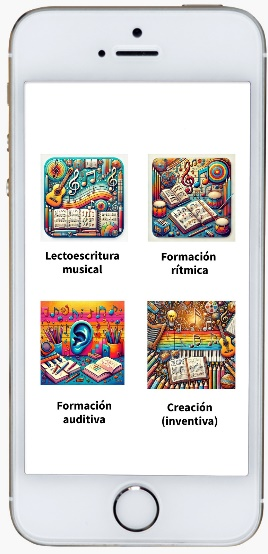
\includegraphics[width=\linewidth]{Fig1.png}
        \caption{Pantalla inicial de la app.}
        \source{Elaboración propia.}
    \end{figure}
\end{minipage}
\hfill
\begin{minipage}[b]{0.30\textwidth}
    \begin{figure}[H]
        \centering
        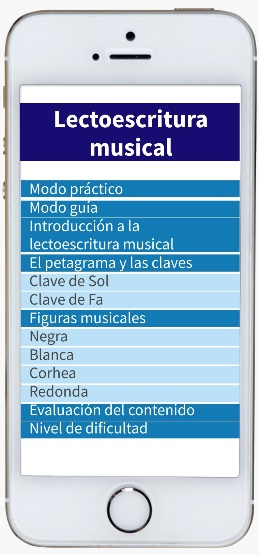
\includegraphics[width=\linewidth]{Fig2.png}
        \caption{Pantalla lectoescritura musical.}
        \source{Elaboración propia.}
    \end{figure}
\end{minipage}

\vspace{0.25cm}

\noindent
\begin{minipage}[b]{0.30\textwidth}
    \begin{figure}[H]
        \centering
        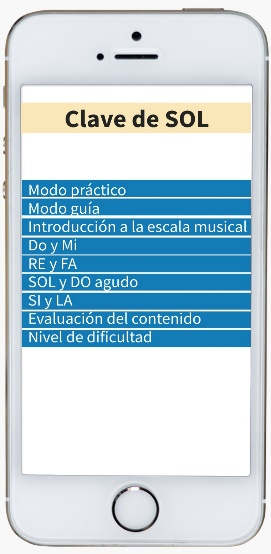
\includegraphics[width=\linewidth]{Fig3.png}
        \caption{ Pantalla lectoescritura musical II.}
        \source{Elaboración propia.}
    \end{figure}
\end{minipage}
\hfill
\begin{minipage}[b]{0.30\textwidth}
    \begin{figure}[H]
        \centering
        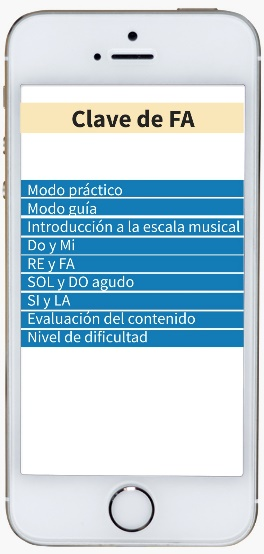
\includegraphics[width=\linewidth]{Fig4.png}
        \caption{Pantalla lectoescritura musical III.}
        \source{Elaboración propia.}
    \end{figure}
\end{minipage}
\clearpage

%---%

\noindent
\begin{minipage}[b]{0.30\textwidth}
    \begin{figure}[H]
        \centering
        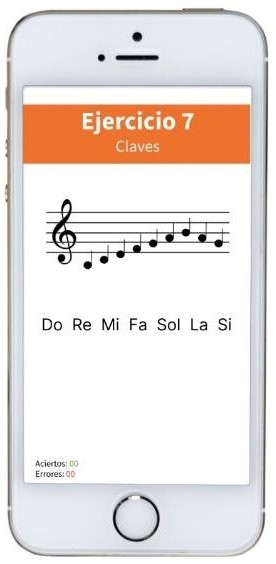
\includegraphics[width=\linewidth]{Fig5.jpg}
        \caption{Pantalla modo ejercicio I.}
        \source{Elaboración propia.}
    \end{figure}
\end{minipage}
\hfill
\begin{minipage}[b]{0.30\textwidth}
    \begin{figure}[H]
        \centering
        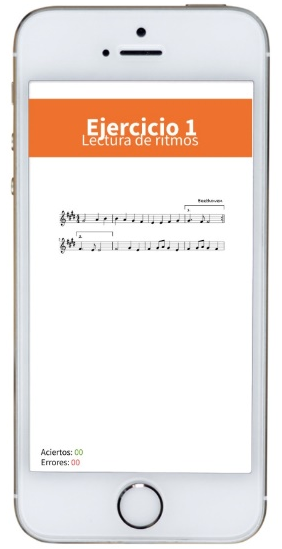
\includegraphics[width=\linewidth]{Fig6.png}
        \caption{Pantalla modo ejercicio II.}
        \source{Elaboración propia.}
    \end{figure}
\end{minipage}

\vspace{0.25cm}

\noindent
\begin{minipage}[b]{0.30\textwidth}
    \begin{figure}[H]
        \centering
        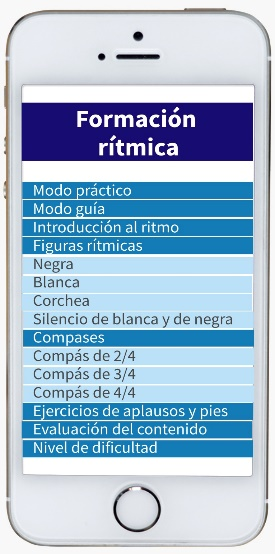
\includegraphics[width=\linewidth]{Fig7.png}
        \caption{Pantalla formación rítmica.}
        \source{Elaboración propia.}
    \end{figure}
\end{minipage}
\hfill
\begin{minipage}[b]{0.30\textwidth}
    \begin{figure}[H]
        \centering
        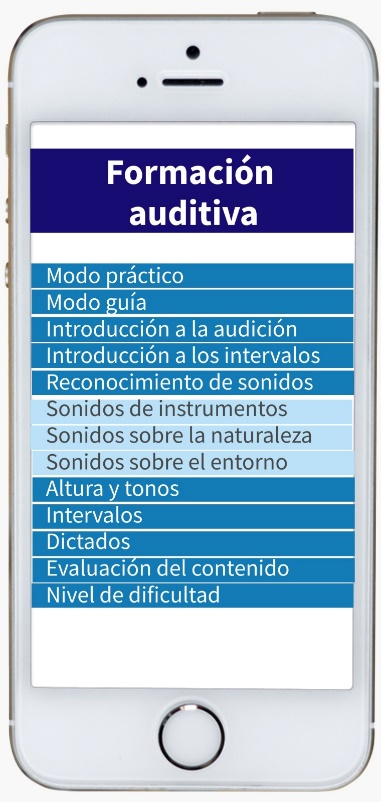
\includegraphics[width=\linewidth]{Fig8.png}
        \caption{Pantalla formación auditiva.}
        \source{Elaboración propia.}
    \end{figure}
\end{minipage}

%----%
\noindent
\begin{figure}[t!]
    \centering
    \begin{minipage}{.3\textwidth}
    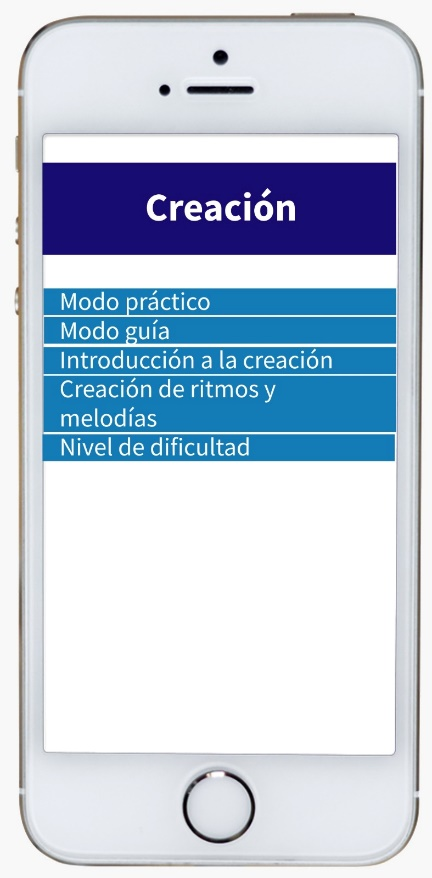
\includegraphics[width=\textwidth]{Fig9.png}
    \caption{Pantalla creación.}
    \source{Elaboración propia.}
    \end{minipage}
    \end{figure}
\end{document}

